\iffalse
\title{2014-ME}
\author{EE24BTECH11020 -  Ellanti Rohith}
\section{me}
\chapter{2014}
\fi
   \item The state of stress at a point is given by $\sigma_x = -6$ $MPa$, $\sigma_y = 4$ $MPa$, and $\tau_{xy} = -8$ $MPa$. The maximum tensile stress (in $MPa$) at the point is \underline{\hspace{2cm}} \hfill{[GATE 2014]}
\\

    \item A block $R$ of mass 100 $kg$ is placed on a block $S$ of mass 150 $kg$ as shown in the figure. Block $R$ is tied to the wall by a massless and inextensible string $PQ$. If the coefficient of static friction for all surfaces is 0.4, the minimum force $F$ (in $kN$) needed to move the block $S$ is \hfill{[GATE 2014]}\\
    \begin{center}
     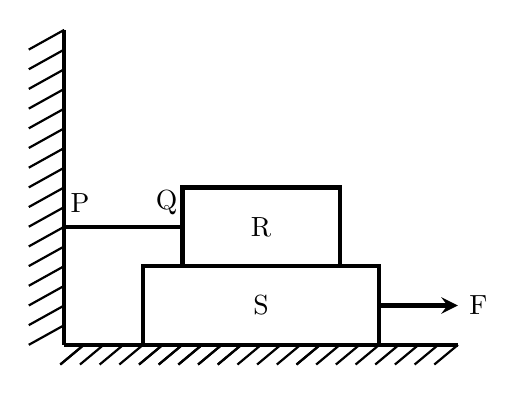
\begin{tikzpicture}
  
    \draw[ultra thick] (-1,4) -- (-1,0);
    \draw[ultra thick] (-1,0) -- (4,0);
\foreach \y in {0.25,0.5,0.75,1,1.25,1.5,1.75,2} {
        \draw[thick] (-1.45,\y-0.25) -- (-1,\y);
    }
   \foreach \y in {0.25,0.5,0.75,1,1.25,1.5,1.75,2} {
        \draw[thick] (-1.45,\y+2-0.25) -- (-1,\y+2);
    }
    \foreach \x in {-1,0,0.25,0.5,0.75,1,1.25,1.5,1.75,2} {
        \draw[thick] (\x-0.05,-0.25) -- (\x+0.25,0);
    }
    \foreach \x in {0,0.25,0.5,0.75,1,1.25,1.5,1.75,2} {
        \draw[thick] (\x-0.05-1,-0.25) -- (\x+0.25-1,0);
    }
     \foreach \x in {0,0.25,0.5,0.75,1,1.25,1.5,1.75} {
        \draw[thick] (\x-0.05+2,-0.25) -- (\x+0.25+2,0);
    }
    \draw[ultra thick] (0,0) rectangle (3,1) node[midway] {S};
    \draw[ultra thick] (0.5,1) rectangle (2.5,2) node[midway] {R};


    \draw[ultra thick] (-1,1.5) -- (0.5,1.5); 
    \draw[ultra thick] (0.5,1.5) -- (0.5,2);\node at (-0.8,1.8) {P};\node at(0.3,1.8) {Q};
    \draw[->, ultra thick,>=stealth] (3,0.5) -- ++(1,0) node[right] {F};
\end{tikzpicture}

    \end{center}

    \begin{multicols}{4}
    \begin{enumerate}
         \item 0.69
        \item 0.88
        \item 0.98
        \item 1.37
    
    \end{enumerate}
       
    \end{multicols}

    \item A pair of spur gears with module 5 $mm$ and a center distance of 450 $mm$ is used for a speed reduction of 5:1. The number of teeth on pinion is \underline{\hspace{2cm}} \hfill{[GATE 2014]}\\

   
    \item Consider a cantilever beam, having negligible mass and uniform flexural rigidity, with length 0.01 $m$. The frequency of vibration of the beam, with a 0.5 $kg$ mass attached at the free tip, is 100 $Hz$. The flexural rigidity (in N$\cdot$m$^2$) of the beam is \underline{\hspace{2cm}} \hfill{[GATE 2014]}\\

    \item An ideal water jet with volume flow rate of 0.05 m$^3$/s strikes a flat plate placed normal to its path and exerts a force of 1000 $N$. Considering the density of water as 1000 $kg/m$ $^3$, the diameter (in $mm$) of the water jet is \underline{\hspace{2cm}} \hfill{[GATE 2014]}\\
 

    \item A block weighing 200 $N$ is in contact with a level plane whose coefficients of static and kinetic friction are 0.4 and 0.2, respectively. The block is acted upon by a horizontal force (in newton) $P = 10t$, where $t$ denotes the time in seconds. The velocity (in $m/s$) of the block attained after 10 seconds is \underline{\hspace{2cm}} \hfill{[GATE 2014]}\\

      \item A slider crank mechanism has slider mass of 10 $kg$, stroke of 0.2 $m$ and rotates with a uniform angular velocity of 10 $rad/s$. The primary inertia forces of the slider are partially balanced by a revolving mass of 6 $kg$ at the crank, placed at a distance equal to crank radius. Neglect the mass of connecting rod and crank. When the crank angle (with respect to slider axis) is 30$\degree$, the unbalanced force (in newton) normal to the slider axis is\underline{\hspace{2cm}} \hfill{[GATE 2014]}
\\
 \item An offset slider-crank mechanism is shown in the figure at an instant. Conventionally, the Quick  Return Ratio (QRR) is considered to be greater than one. The value of QRR is 

 
\begin{centering}
  \begin{tikzpicture}
   \draw[thick] (3.75,10.75) arc[start angle=90, end angle=-90, radius=0.374];
    \draw[thick] (3,10.75) -- (3.75,10.75);
    \draw[thick] (3,10) -- (3.75,10);
    \draw[ultra thick] (3,11) -- (3,9.5);
    \draw[thick] (3,10.5) -- (2.75,10.75);
    \draw[thick] (3,10) -- (2.75,10.25);
    \draw[thick] (3,10.25) -- (2.75,10.5);
    \draw[thick] (3,9.75) -- (2.75,10);
    \draw[thick] (3,10.75) -- (2.75,11);
   \node at (3.5,11.5) {20 $mm$};\node at (7,12) {40 $mm$};\node at (11.75,11) {10 $mm$};
    
    \draw[thick] (8.75,11.25) -- (8.5,11);\draw[thick] (8.75,11) -- (9,11.25);\draw[thick] (9,11) -- (9.25,11.25); \draw[thick] (9.25,11.25) -- (9,11);\draw[thick] (9.25,11) -- (9.5,11.25);\draw[thick] (9.5,11) -- (9.75,11.25);\draw[thick] (9.75,11) -- (10,11.25);
    \draw[thick] (8.75,11.25) -- (8.75,12);
    \draw[thick] (3.5,10.5) -- (4.75,11.75);
    \draw[thick] (4.75,11.75) -- (9.5,11.625);
    \draw[ultra thick] (8.5,11.25) -- (10.25,11.25);
    \draw[thick] (8.75,11.25) -- (8.75,12);
    \filldraw(9.5,11.625) circle (2pt) {};
    \filldraw (4.75,11.75)circle (2pt) {};\filldraw (3.5,10.5)circle (2pt) {};
    \draw[thick] (8.75,12) -- (10,12);
    \draw[thick] (10,12) -- (10,11.25);

    \draw[dashed, thick] (9.625,11.625) -- (11,11.625);
    \draw[dashed, thick] (3.5,10.45) -- (11.5,10.45);
    \draw[<->, thick, >=Stealth] (11,11.625) -- (11,10.5);
   
\end{tikzpicture}
   
\end{centering}\hfill{[GATE 2014]}
 \\

  
\item A rigid uniform rod $AB$ of length $L$ and mass $m$ is hinged at $C$ such that $AC = L/3$, $CB = 2L/3$. Ends $A$ and $B$ are supported by springs of spring constant $k$. The natural frequency of the system is given by \\


\begin{centering}
\begin{tikzpicture}
 
    \draw[line width=1.1pt] (1.25,13.25) -- (2.5,13.25);
    \draw[line width=1.1pt] (2.5,13.25) -- (3.75,13.25);
    \draw[line width=1.1pt] (7.5,13.25) -- (10,13.25);

 
    \draw[line width=1.1pt] (2.5,13.25) -- (2.5,12.5);
    \draw[line width=1.1pt] (2.5,12.5) -- (3,12);
    \draw[line width=1.1pt] (3,12) -- (2.5,11.5);
    \draw[line width=1.1pt] (2.5,11.5) -- (3,11);
    \draw[line width=1.1pt] (3,11) -- (2.5,10.5);
    \draw[line width=1.1pt] (8,13.25) -- (10,13.25);
    \draw[line width=1.1pt] (2.5,10.5) -- (2.5,10);
    \draw[line width=1.1pt] (8.75,13.25) -- (10,13.25);

    
    \draw[line width=1.1pt] (8.75,13.25) -- (8.75,12.5);
    \draw[line width=1.1pt] (8.75,12.5) -- (9.25,12);
    \draw[line width=1.1pt] (9.25,12) -- (8.75,11.5);
    \draw[line width=1.1pt] (8.75,11.5) -- (9.25,11);
    \draw[line width=1.1pt] (9.25,11) -- (8.75,10.5);
    \draw[line width=1.1pt] (8.75,10.5) -- (8.75,10);

   
   \draw[line width=1.4pt] (2.5,10) -- (8.75,10);
\draw[line width=1.6pt] (3.25,8.75) -- (2.5,8.75) [->, >=Stealth];
\node at (3.75,8.75) {\footnotesize L/3};
\draw[line width=1.6pt] (4.2,8.75) -- (5,8.75) [->, >=Stealth];
\draw[line width=1.6pt] (6.25,8.75) -- (5,8.75) [->, >=Stealth];
\draw[line width=1.6pt] (7.75,8.75) -- (8.75,8.75) [->, >=Stealth];
\node at (7,8.75) {\footnotesize 2L/3};


 \draw[thick] (4.65,10) -- (4.65,9.75);
    \draw[thick] (5.35,10) -- (5.35,9.75); 
    \draw[thick] (5.35,10) arc (0:180:0.35); 
    \draw[thick] (5.35,9.75) -- (4.65,9.75);
    \draw[fill=white] (5, 10) circle (0.1); 

    \draw[thick] (5.1,9.75)--(4.9,9.5);\draw[thick] (4.9,9.75)--(4.7,9.5);\draw[thick] (4.7,9.75)--(4.5,9.5);\draw[thick] (5.3,9.75)--(5.1,9.5);
  
    \node at (8.25,11.5) {$k$};
    \node at (2,11.5) {$k$};
    \node at (2.25,9.75) {A};
    \node at (9,9.75) {B};
    \node at (5.25,10.5) {C};
\draw[thick] (2.5,9) -- (2.5,8.5);
\draw[thick] (5,9) -- (5,8.5);
\draw[thick] (8.75,9) -- (8.75,8.5);

    \draw[thick] (1.75,13.25) -- (2.5,13.75);
    \draw[thick] (2.5,13.25) -- (3.25,13.75);
    \draw[thick] (3.25,13.25) -- (4,13.75);
    \draw[thick] (8,13.25) -- (8.75,13.75);
    \draw[thick] (8.75,13.25) -- (9.5,13.75);
    \draw[thick] (9.5,13.25) -- (10.25,13.75);

  
\end{tikzpicture}


\end{centering}    
   
\hfill{[GATE 2014]}
    \begin{multicols}{4}
    \begin{enumerate}
        \item $\sqrt{\frac{k}{2m}}$
        \item $\sqrt{\frac{k}{m}}$
        \item $\sqrt{\frac{2k}{m}}$
        \item $\sqrt{\frac{5k}{m}}$
    \end{enumerate}
    \end{multicols}
    \item A hydrodynamic journal bearing is subject to 2000 $N$ load at a rotational speed of 2000 rpm. Both bearing bore diameter and length are 40 $mm$. If radial clearance is 20 $\mu m$ and bearing is lubricated with an oil having viscosity 0.03 $Pa.s$, the Sommerfeld number of the bearing is \underline{\hspace{2cm}}\hfill{[GATE 2014]}
   \\
    

    \item A 200 $mm$ long, stress-free rod at room temperature is held between two immovable rigid walls. The temperature of the rod is uniformly raised by 250$\degree C$. If the Young's modulus and coefficient of thermal expansion are 200 $GPa$ and $1 \times 10^{-5}/ \degree C$, respectively, the magnitude of the longitudinal stress (in $MPa$) developed in the rod is \underline{\hspace{2cm}}\hfill{[GATE 2014]}
  \\
  
\item 1.5 kg of water is in saturated liquid state at 2 bar ($v_f = 0.001061$ m$^3 /kg$, $u_f = 504.0$ $kJ/kg$, $h_f = 505$ $kJ/kg$). Heat is added in a constant pressure process till the temperature of water reaches 400$\degree C$ ($v = 1.5493$ m$^3 /kg$, $u = 2967.0$ $kJ/kg$, $h = 3277.0$ /, $kJ/kg$). The heat added (in $kJ$) in the process is \underline{\hspace{2cm}}\hfill{[GATE 2014]}
 \\
    
 \item Consider one dimensional steady state heat conduction across a wall (as shown in figure below) of thickness $30 \ \text{mm}$ and thermal conductivity $15 \ \text{W/m.K}$. At $x = 0$, a constant heat flux, $q'' = 1 \times 10^5 \ \text{W/m}^2$ is applied. On the other side of the wall, heat is removed from the wall by convection with a fluid at $25^\circ \text{C}$ and heat transfer coefficient of $250 \ \text{W/m}^2\cdot\text{K}$. The temperature (in $^\circ \text{C}$), at $x = 0$ is \underline{\hspace{2cm}}\hfill{[GATE 2014]}

\begin{center}
 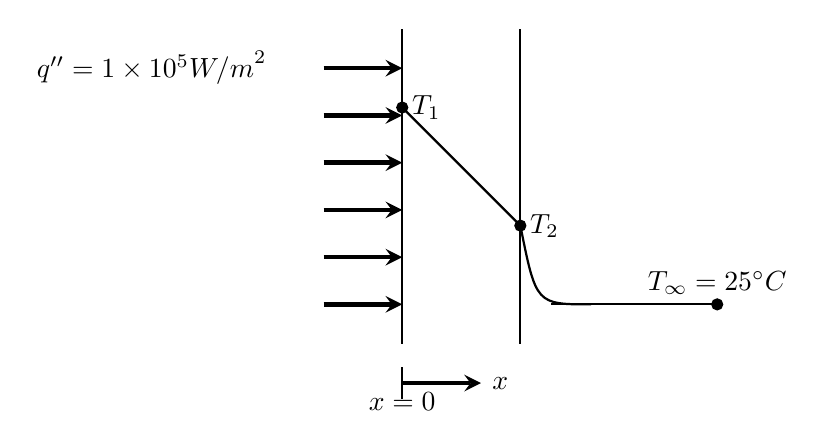
\begin{tikzpicture}
   
    \draw[thick] (0,-2) -- (0,2);
\draw[thick] (1.5,-2) -- (1.5,2);
  
    \foreach \y in {-1.5, -0.9, -0.3, 0.3, 0.9, 1.5} {
        \draw[->, ultra thick,>=stealth] (-1, \y) -- (0, \y);
    }

   
    \node[left] at (-1.6, 1.5) {$q'' = 1 \times 10^5  \text{ W/m}^2$};

    
    \filldraw (0, 1) circle (2pt) node[right] {$T_1$};
    \filldraw (1.5, -0.5) circle (2pt) node[right] {$T_2$};
    \filldraw (4, -1.5) circle (2pt) node[above] {$T_\infty = 25^\circ\text{C}$};

   
    \draw[thick] (0,1) -- (1.5,-0.5); 
    \draw[thick] (1.5,-0.5) .. controls(1.7,-1.5)..(2.4,-1.5); 
\draw[thick] (4,-1.5)--(1.89,-1.5);
   
   \draw[->, ultra thick, >=stealth] (0, -2.5) -- (1, -2.5) node[right] {$x$};
    
  
    \draw[thick] (0, -2.3) -- (0, -2.7);
    
   
    \node[below] at (0, -2.5) {$x=0$};
\end{tikzpicture}
    \end{center}

 
